\documentclass[11pt]{article}
%Homework 01 |065|=)
\usepackage{amsmath,amssymb}
\usepackage{graphicx}
\usepackage[colorlinks=true,citecolor=black,linkcolor=black,urlcolor=blue]{hyperref}
\usepackage{tikz,graphics,color,fullpage,float,epsf,caption,subcaption}
\usepackage[utf8]{inputenc}
\usepackage{float}
\graphicspath{ {images/} }
\title{\textbf{Polynomial Systems Solving}}
\author{Burak ŞENER\\
        Mehmet PEKMEZCİ\\
		Mustafa Mert ERGİN\\
		Şefik Temel
		}
\date{}
\begin{document}
\maketitle
\begin{abstract}
\emph{This work is a survey on the subject Polynomial Systems Solving. First , Polynomial Systems definition is studied , then their solution techniques are studied, finally application areas are discussed. }
\end{abstract}

\section{Introduction}

\subsection{Polynomial}
 A polynomial is a mathematical expression involving a sum of powers in one or more variables (indeterminates) multiplied by coefficients. A polynomial of order/degree $\mathbf{d}$  in one variable ($\mathbf{x \in C}$) (i.e., a univariate polynomial) with constant coefficients ($\mathbf{a_i \in Q}$ ) is given by \cite{wolframPolynomial}
\begin{equation}
    P(x)=a_{0}+a_{1}x+a_{2}{x}^2+\cdots+a_{d}{x}^d
\end{equation}

\subsubsection{Properties of Polynomials}

Properties of polynomials are as follows :
\begin{enumerate}
\item A polynomial may not have a term with negative and fractional exponent ($\mathrm{x^{-n}}$ and $\mathrm{x^{1/n}}$ ).
\item $\mathrm{x \in C}$ and $\mathrm{a_i \in Q}$
\item Every term ( $\mathbf{a_ix^i}$ ) may be called as monomial (in some books only $\mathbf{x^i}$ is called as monomial).
\end{enumerate}

\subsubsection{Solution of Polynomials}

 Polynomials of orders one to four are solvable using only rational operations and finite root extractions. \cite{wolframPolynomial}
\begin{enumerate}
\item A first-order equation is trivially solvable.
\item A second-order equation is soluble using the quadratic equation.
\item A third-order equation is solvable using the cubic equation.
\item A fourth-order equation is solvable using the quartic equation.
\item It was proved by Abel and Galois using group theory that general equations of fifth and higher order cannot be solved rationally with finite root extractions (Abel's impossibility theorem).
\end{enumerate}

Solutions of the general quintic equation may be given in terms of \textbf{Jacobi theta functions} or \textbf{hypergeometric functions} in one variable.\cite{wolframPolynomial}
\begin{enumerate}
\item Hermite and Kronecker proved that higher order polynomials are not soluble in the same manner.
\item Klein showed that the work of Hermite was implicit in the group properties of the icosahedron. Klein's method of solving the quintic in terms of hypergeometric functions in one variable can be extended to the sextic, but for higher order polynomials, either hypergeometric functions in several variables or "Siegel functions" must be used (Belardinelli 1960, King 1996, Chow 1999).
\item In the 1880s, Poincaré created functions which give the solution to the nth order polynomial equation in finite form. These functions turned out to be "natural" generalizations of the elliptic functions.
\end{enumerate}




\subsection{Polynomial System}

A system of (multivariate) polynomial equations is a set of simultaneous equations $\mathrm{f_{1}}$  = 0, ..., $\mathrm{f_{m}}$ = 0 where the $\mathrm{f_{i}}$ are polynomials in several variables, say $\mathrm{x_{1}}$, ..., $\mathrm{x_{n}}$, over some field k (usually $\mathbb{C}$ or $\mathbb{R}$ ).
\cite{wikipediaSystemofPolynomialEquations}.

In abstract algebra books,  a \textbf{Polynomial System} is called as \textbf{Polynomial Ring} or \textbf{Polynomial Algebra}. \cite{wolframPolynomial} Abstract algebraic notions are explained in the section 2.

A \textbf{Univariate Polynomial System}  (coefficients  $\mathrm{a_{ij} \in R}$  and i,j,n $\mathrm{\in N}$) may be given as m equations:

\begin{equation}
   \begin{cases}
    a_{10}+a_{11}x+a_{12}x^2+a_{13}x^3+a_{14}x^4+\ldots+a_{1d}x^d=0 \\
    a_{20}+a_{21}x+a_{22}x^2+a_{13}x^3+a_{14}x^4+\ldots+a_{2d}x^d=0 \\
    a_{30}+a_{31}x+a_{12}x^2+a_{13}x^3+a_{14}x^4+\ldots+a_{3d}x^d=0 \\
    \vdots \\
    a_{m0}+a_{m1}x+a_{m2}x^2+a_{m3}x^3+a_{m4}x^4+\ldots+a_{md}x^d=0 \\
  \end{cases}
\end{equation}


A \textbf{Bivariate Polynomial System}  (variables  $\mathrm{x,y \in R}$ ,  coefficients  $\mathrm{a_{ij} \in R}$  and i,j,n $\mathrm{\in N}$) may be given as m equations :

\begin{equation}
   \begin{cases}
    a_{00}+a_{01}xy+a_{02}xy^2+a_{03}xy^3+\ldots+a_{0(d \times d)}x^dy^d=0 \\
    a_{10}+a_{11}xy+a_{12}xy^2+a_{13}xy^3+\ldots+a_{1(d \times d)}x^dy^d=0 \\
    a_{20}+a_{21}xy+a_{22}xy^2+a_{23}xy^3+\ldots+a_{2(d \times d)}x^dy^d=0 \\
    \vdots \\
    a_{m00}+a_{m11}xy+a_{m12}xy^2+a_{m13}xy^3+\ldots+a_{m(d \times d)}x^dy^d=0 \\
  \end{cases}
\end{equation}


A \textbf{Multivariate Polynomial System}  (N variables  $\mathrm{x_1 \ldots x_N \in R}$ ,  coefficients  $\mathrm{a_{ij} \in R}$  and i,j,n $\mathrm{\in N}$) may be given as m equations :

\begin{equation}
   \begin{cases}
    a_{00}+\sum_{i_1,\ldots,i_n}^{d}{a_{0i}{x_1}^{i_1}{x_2}^{i_2} \ldots {x_n}^{i_n} }=0 \\
    a_{10}+\sum_{i_1,\ldots,i_n}^{d}{a_{1i}{x_1}^{i_1}{x_2}^{i_2} \ldots {x_n}^{i_n} }=0 \\
    \vdots \\
    a_{m0}+\sum_{i_1,\ldots,i_n}^{d}{a_{mi}{x_1}^{i_1}{x_2}^{i_2} \ldots {x_n}^{i_n} }=0 \\
  \end{cases}
\end{equation}


\section{Abstract Algeraic Notions}
\cite{abstractAlgebraBook}
\section{Geometrical Meaning}

An affine variety $\mathrm{V(f_1 \ldots f_s)	\subset k^n}$ is the set of all solutions of the system of equations \\
 $\mathrm{f_1(x_1 \ldots x_n) = \ldots = f_s(x_1 \ldots x_n)}$ = 0. We will use the letters V,W,etc. to denote affine varieties. \cite{coxLittleOshea}
 \newline
 \newline
The conic sections studied in analytic geometry (circles, ellipses, parabolas) are affine varieties. Likewise, graphs of polynomial functions are affine varieties
[the graph of $\mathbf{y= f(x) \text{} \text{ is } \text{} V(y - f(x))}$].
Although not as obvious, graphs of rational functions are also affine varieties. For example, consider the graph of $\mathbf{y= \frac{x^3 -1}{x}}$ :

\begin{figure}[H]
  \begin{center}
    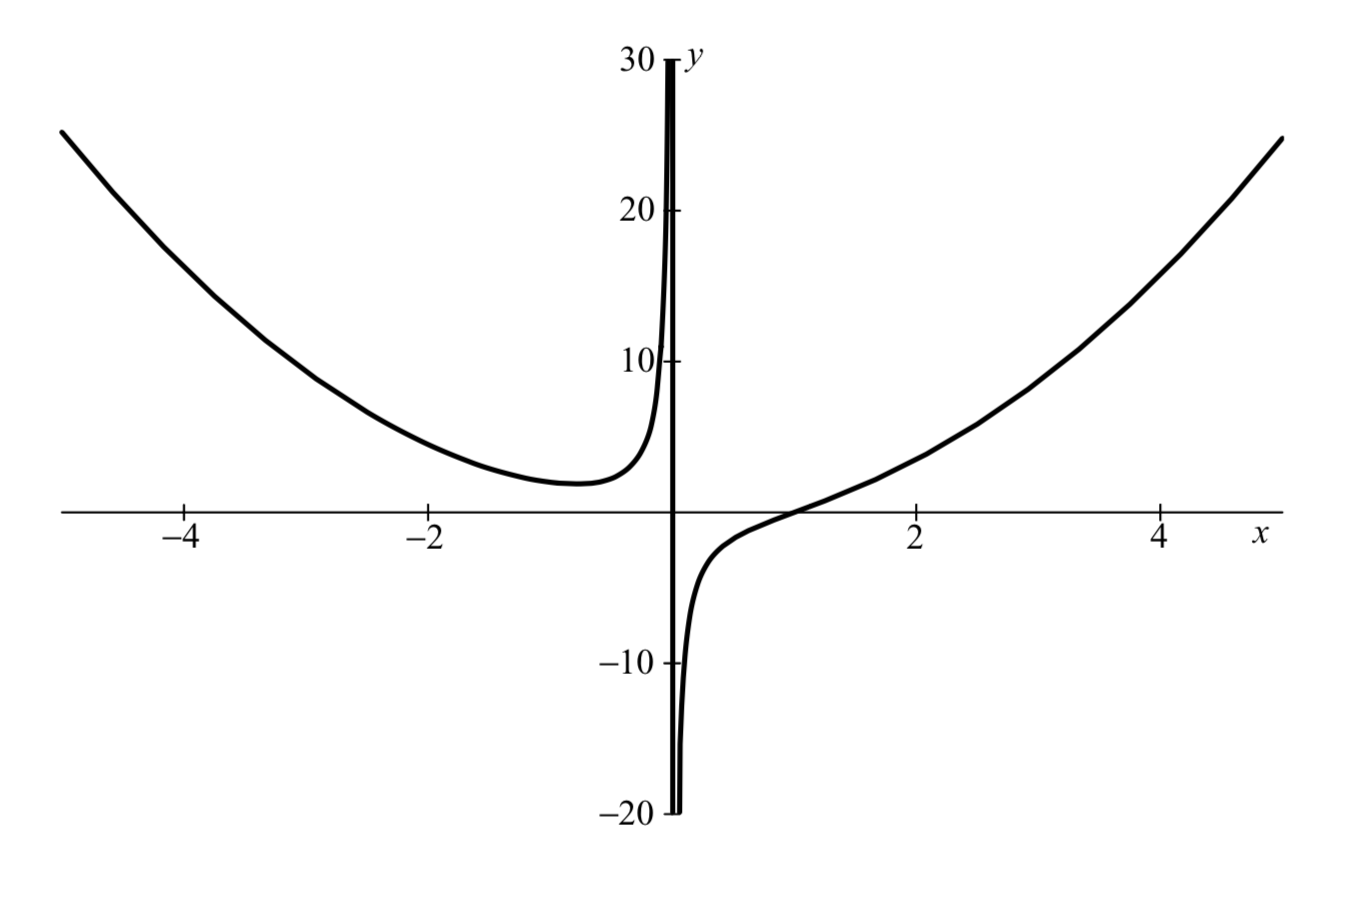
\includegraphics[width=0.50\textwidth]{conic.png}
    \caption{}
    \label{fig: }
  \end{center}
\end{figure}

3-dimensional space example. A nice affine variety is given by
paraboloid of revolution $\mathbf{V(z - x^2 - y)}$, which is obtained by rotating the parabola $\mathbf{z= x^2}$ about the z-axis.
This gives us the picture:

\begin{figure}[H]
  \begin{center}
    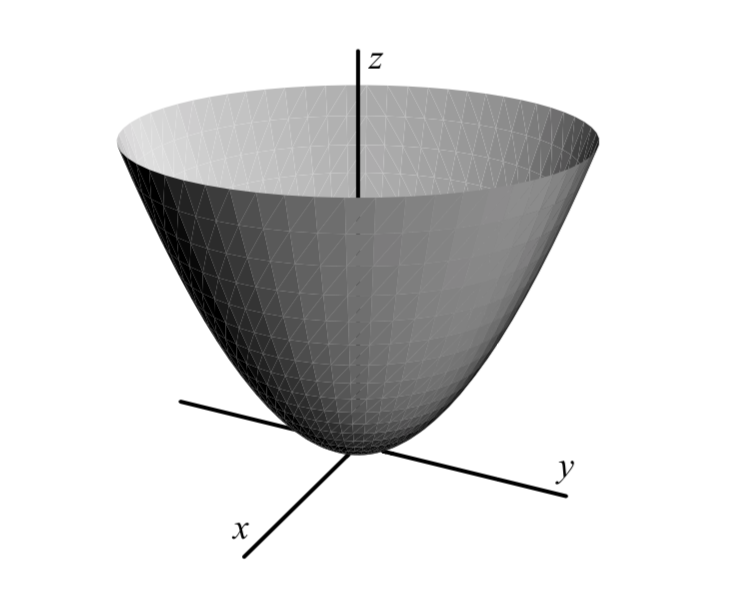
\includegraphics[width=0.50\textwidth]{threedimensinoal.png}
    \caption{}
    \label{fig: }
  \end{center}
\end{figure}

A much more complicated surface is given by $\mathbf{V(x^2 - y^2z^2 + z^3)}$:

\begin{figure}[H]
  \begin{center}
    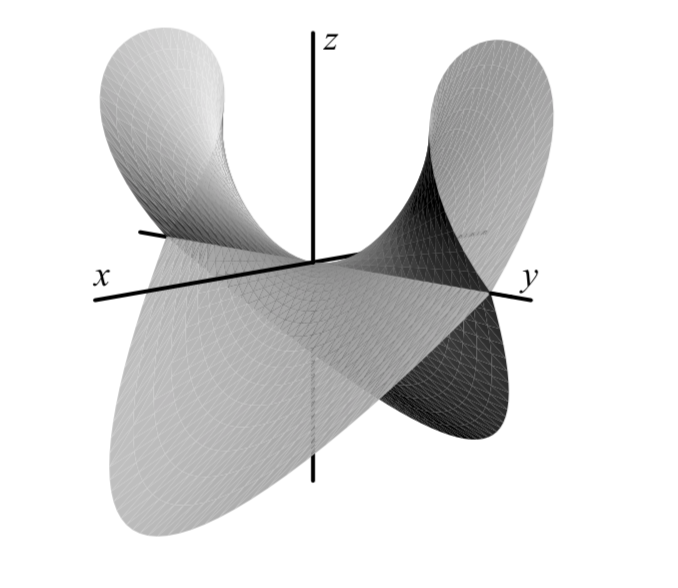
\includegraphics[width=0.50\textwidth]{complicated.png}
    \caption{}
    \label{fig: }
  \end{center}
\end{figure}

\section{Polynomial Systems Solution Methods}


\section{Solver Software}

\section{Applications}
Systems of polynomial equations show up in many applications areas such as robotics (kinematics,motion planning, collision detection, etc.), computer vision (object modeling, surface fitting,recognition, etc.), graphics, geometric modeling (curve and surface intersections), computer-aided design, mechanical design, and chemical equilibrium systems. \cite{yanbinjiaArticle}
\subsection{Robotics}
System of polynomial equations may use to model a robot arm. If  ($\mathbf{x_i, y_i}$) is the coordinates of some joint,  ($\mathbf{x_i+1, y_i+1}$) is the coordinates of the next joint (or the hand) and the segment has length Li then we get the equation \cite{richterArticle}
\begin{figure}[H]
  \begin{center}
    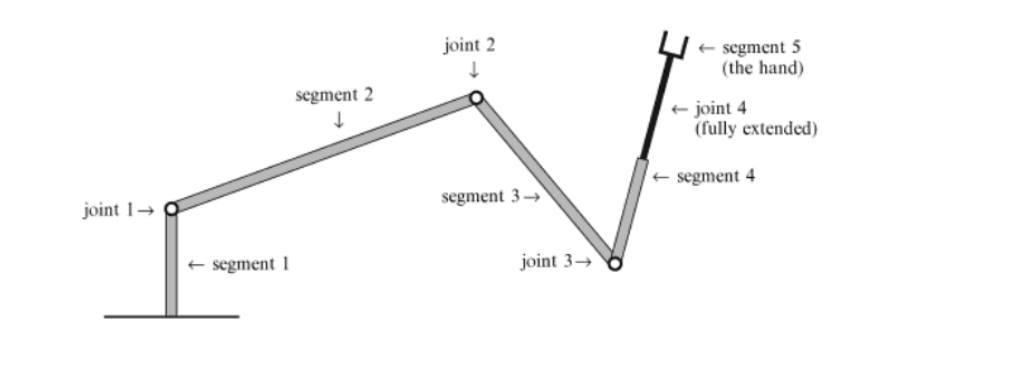
\includegraphics[width=0.70\textwidth]{robotarm.png}
    \caption{Robot Arm}
    \label{fig: Robot Arm}
  \end{center}
\end{figure}

 \begin{equation}
    (x_{i+1}-x_i)^2 + (y_{i+1}-y_i)^2=L_i^2
\end{equation}
Note that the angle at the i-th joint can be computed from the equations
 \begin{equation}
    x_{i+1}-x_i = L_i \cos(\theta_i)
\end{equation}
 \begin{equation}
    y_{i+1}-y_i = L_i \sin(\theta_i)
\end{equation}

\subsection{Geometry}
Many statements in Euclidean geometry can be formulated as result about systems of polynomial equations.\cite{richterArticle}

\textbf {Example:} Euclidean geometry says that \textit{the bisectors of the three sides of a triangle meet in one point.}

One vertex, A, of the triangle can be assumed to be the origin and another, B, to have coordinates (c, 0), without loss of generality. The third vertex, C, has coordinates (a,b).
The bisectors of AB and BC meet in some point, with coordinates (x1, y1). We get the following equations
\begin{equation}
    x_1- \frac {c}{2}=0
\end{equation}
\begin{equation}
    \frac {c-a}{b} \cdotp x_1 - y_1 + \frac {a^2 + b^2 - c^2}{2b} = 0
\end{equation}

Similarly, if (x2,y2) are the coordinates of the intersection of the bisectors of AB and AC we have
\begin{equation}
    x_2- \frac {c}{2}=0
\end{equation}
\begin{equation}
    \frac {a}{b} \cdotp x_2 + y_2 - \frac {b^2 + a^2}{2b} = 0
\end{equation}

\section{Conclusion}


\begin{thebibliography}{1}
\bibitem{berndStrumfelsBook}
  Strumfels Bernd,
  \textit{Solving Systems of Polynomial Equations},
   American Mathematical Society , Conference Board of Mathematical Sciences,
   Berkeley,CA,
   2002.
\bibitem{dineshManocaArticle}
  Manocha Dinesh,
  \textit{Solving Systems of Polynomial Equations},
   IEEE Computer Graphics and Applications
   University of North Carolina,
   1994.
\bibitem{hybridMethodArticle}
  L.H. Zhi and Y. Notake and H. Kai and M.-T. Noda and K.I. Shiraishi,
  \textit{Hybrid Method for Solving Polynomial Equations},
   Proceedings of the Asian Technology Conference in Mathematics, pp.492-501, Guangzhou, China, 1999.
\bibitem{gregoryBardThesis}
  Bard Gregory,
  \textit{Algorithms for Solving Linear and Polynomial Systems of Equations Over Finite Fields With Applications to Cryptanalysis},
   University of Maryland PHD Thesis,
   2007.
\bibitem{bettaleLukArticle}
  Luk Bettale 1 , Jean-Charles Faugère, Ludovic Perret,
  \textit{Solving multivariate polynomial systems over finite fields : Hybrid approach},
   Journées Nationales du Calcul Formel,
   UPMC, CNRS, INRIA Paris-Rocquencourt,
   2002.

\bibitem{morhacArticle}
   M. MORHAC,
  \textit{One-Modulus Residue Arithmetic Algorithm to Solve Linear Equations Exactly},
   Institute of Physics, Slovak Academy of Sciences
   Bratislava, Slovakia,
   1994.
\bibitem{emirisReport}
  I.Z. Emiris, A. Mantzaflaris, E. Tsigaridas,
  \textit{On the Bit Complexity of Solving Bilinear Polynomial Systems},
   Johan Radon Institute for Computational Mathematics,
   Austrian Academy Of Sciences,
   2016.
\bibitem{verscheldeArticle}
  Jan Verschelde,
  \textit{Homotopy Methods for Solving Polynomial Systems},
   ISSAC’05
   Beijing, China,
   2005.
\bibitem{courtoisaArticle}
  Nicolas Courtois , Alexander Klimov  , Jacques Patarin ,  Adi Shamir
  \textit{Efficient Algorithms for Solving Overdefined Systems of Multivariate Polynomial Equations},
   International Conference on the Theory and Applications of Cryptographic Techniques
   EUROCRYPT-2000,
   2000.
\bibitem{lazardArticle}
  Daniel Lazard,
  \textit{Thirty years of Polynomial System Solving, and now?},
   Journal of Symbolic Computation ,
   UPMC Univ. Paris, France,
   2008.
\bibitem{chenThesis}
  Changbo Chen,
  \textit{Solving Polynomial Systems via Triangular Decomposition},
   PHD Thesis
   The University of Western Ontario,
   2011.
\bibitem{faugereArticle}
  Jean-Charles Faugère, Pierrick Gaudry, Louise Huot, Guénaël Renault,
  \textit{Polynomial Systems Solving by Fast Linear Algebra},
   HAL <hal-00816724v1>,
   2013.
\bibitem{bondyfalatArticle}
  Didier Bondyfalat, Bernard Mourrain ,Victor Y. Pan
  \textit{Controlled iterative methods for solving polynomial systems},
   ISSAC 98 ,
   1998.
\bibitem{marinariArticle}
  M. G. MARINARI, H. M. MÖLLER, AND T. MORA
  \textit{ON MULTIPLICITIES IN POLYNOMIAL SYSTEM SOLVING},
   TRANSACTIONS OF THE AMERICAN MATHEMATICAL SOCIETY,
   1996.
\bibitem{chenArticle}
  Changbo Chen, Marc Moreno Maza,
  \textit{Algorithms for computing triangular decomposition of polynomial systems},
   Journal of Symbolic Computation,
   2012.
\bibitem{yienliArticle}
  Tien-Yien Li,
  \textit{SOLVING POLYNOMIAL SYSTEMS BY POLYHEDRAL HOMOTOPIES},
   TAIWANESE JOURNAL OF MATHEMATICS,
   1999.
\bibitem{duffArticle}
  Timothy Duff, Cvetelina Hill , Anders Jensen, Kisun Lee, Anton Leykin, Jeff Sommars,
  \textit{Solving polynomial systems via homotopy continuation and monodromy},
   CoRR,
   2017.
\bibitem{sommeseArticle}
  Andrew J. Sommese , Jan Verschelde , Charles W. Wampler ,
  \textit{Solving Polynomial Systems Equation by Equation},
   Dickenstein A., Schreyer FO., Sommese A.J. (eds) Algorithms in Algebraic Geometry,
   2006.
\bibitem{batesArticle}
  Dan Bates,
  \textit{Course Notes for Math 676: Computational Algebraic Geometry Spring 2009},
   Colorado State University,
   2009.
\bibitem{mouArticle}
  Chenqi Mou,
  \textit{Solving Polynomial Systems over Finite Fields:Algorithms, Implementation and Applications},
   HAL,
   Université Pierre et Marie Curie,
   2013.
\bibitem{alessioArticle}
  Caminata Alessio , Gorla Elisa.
  \textit{Solving Multivariate Polynomial Systems and an Invariant from Commutative Algebra. },
   2017.
\bibitem{abstractAlgebraBook}
  Karl-Heinz Fieseler,
  \textit{Groups, Rings and Fields },
   Upsalla
   2010.
\bibitem{richterArticle}
  Johan Richter,
  \textit{Systems of polynomial equations},
   2013.
\bibitem{wikipediaSystemofPolynomialEquations}
  \textit{ https://en.wikipedia.org/wiki/System\_of\_polynomial\_equations},
   Wikipedia,2018.

\bibitem{wolframPolynomial}
  \textit{ http://mathworld.wolfram.com/Polynomial.html},
   Wolfram,2018.
 \bibitem{yanbinjiaArticle}
  \textit{ https://pdfs.semanticscholar.org/295c/9b5d5e1120fdb3d5cf2386d8f6a92884d9f5.pdf},
   Yan-Bin Jia,2017.
\bibitem{coxLittleOshea}
   Cox, Little, O'Shea,
   \textit{Ideals, Varieties, and Algorithms Book},
\end{thebibliography}

\end{document}
